\newpage	
	\section{Листок 3}
	
		\subsection{1}
		A)\\
		Рефлексивность: $(x, y) \preccurlyeq_1 (x, y)$, так как $x \leqslant x, y \leqslant y$\\
		Антисимметричность: $(x_1, y_1) \preccurlyeq_1 (x_2, y_2)  \Longrightarrow  x_1 \leqslant x_2, y_1 \leqslant y_2$ ;\\ 
		$(x_2, y_2) \preccurlyeq_1 (x_1, y_1)  \Longrightarrow  x_2 \leqslant x_1, y_2 \leqslant y_1$ \\
		$\Longrightarrow$ $x_1 = x_2, y_1 = y_2 \Longrightarrow (x_1, y_1) = (x_2, y_2)$\\
		Транзитивность: $(x_1, y_1) \preccurlyeq_1 (x_2, y_2)  \Longrightarrow  x_1 \leqslant x_2, y_1 \leqslant y_2$; \\
		$(x_2, y_2) \preccurlyeq_1 (x_3, y_3)  \Longrightarrow  x_2 \leqslant x_3, y_2 \leqslant y_3$ \\
		$\Longrightarrow$ $x_1 \leqslant x_3, y_1 \leqslant y_3 \Longrightarrow (x_1, y_1) \preccurlyeq_1 (x_3, y_3)$
		\\
		Откуда отношение является отношением частичного порядка. При это не является отношением линейного порядка, так как\\
		$(1;2) !\preccurlyeq_1 (2;1)$ и $(2;1) !\preccurlyeq_1 (1;2)$
		\\ \\
		B)\\
		Заметим, что если ($\preccurlyeq_2$) - отношение частичного порядка, то
		$(1;2) \preccurlyeq_2 (2;1)$ и $(2;1) \preccurlyeq_2 (1;2)$, откуда должно быть (1;2) = (2;1), что не так $\Longrightarrow$ это не отношение частичного порядка, откуда и не линейного.
		\\ \\
		C)\\
		Заметим, что если ($\preccurlyeq_3$) - отношение частичного порядка, то
		$(1;2) \preccurlyeq_3 (1;2)$, но $max(1, 2) = 2; min(1, 2) = 1$, откуда $max(1, 2) > min(1, 2)$, что противоречит $max(1, 2) \leqslant min(1, 2)$, откуда это не отношение частичного порядка, соотв. и не линейного.
		\\ \\
		D)\\
		Заметим, что если ($\preccurlyeq_4$) - отношение частичного порядка, то
		$(1;2) \preccurlyeq_4 (2;1)$ и $(2;1) \preccurlyeq_4 (1;2)$, откуда должно быть (1;2) = (2;1), что не так $\Longrightarrow$ это не отношение частичного порядка, откуда и не линейного.
		\\ \\
		E)\\
		Рефлексивность: $(x, y) \preccurlyeq_5 (x, y)$, так как $x = x, y = y$\\
		Антисимметричность: $(x_1, y_1) \preccurlyeq_5 (x_2, y_2)  \Longrightarrow  x_1 \leqslant x_2, y_1 \leqslant y_2$ ;\\ 
		$(x_2, y_2) \preccurlyeq_5 (x_1, y_1)  \Longrightarrow  x_2 \leqslant x_1, y_2 \leqslant y_1$ \\
		$\Longrightarrow$ $x_1 = x_2, y_1 = y_2 \Longrightarrow (x_1, y_1) = (x_2, y_2)$\\
		Транзитивность: $(x_1, y_1) \preccurlyeq_5 (x_2, y_2)  \Longrightarrow  x_1 \leqslant x_2, y_1 \leqslant y_2$; \\
		$(x_2, y_2) \preccurlyeq_5 (x_3, y_3)  \Longrightarrow  x_2 \leqslant x_3, y_2 \leqslant y_3$ \\
		$\Longrightarrow$ $x_1 \leqslant x_3, y_1 \leqslant y_3 \Longrightarrow (x_1, y_1) \preccurlyeq_5 (x_3, y_3)$
		\\ \\
		Откуда отношение - частиного порядка. При этом оно и линейного порядка, так как для пары $(x_1, y_1)$ и $(x_2, y_2)$ верно, что либо ($x_1 < x_2$ или $x_2 < x_1$) либо ($x_1 = x_2$ и ($y_1 < y_2$ или $y_2 < y_1$)) либо ($x_1 = x_2$ и $y_1 = y_2$), откуда $(x_1, y_1) \preccurlyeq_5 (x_2, y_2)$ или $(x_2, y_2) \preccurlyeq_5 (x_1, y_1)$\\
		
		\newpage
		\subsection{2}
		Пусть элементы A, B, C. Тогда есть $1 + 6 + 3*2 + 6 = 19$ отношения частичного порядка:\\
		1)$A \quad B \quad C$\\
		\begin{center}
			\begin{tikzpicture}
				\node (a) at (1,1.7) {$A$};
				\node (b) at (2,0) {$B$};
				\node (c) at (0,0) {$C$};
			\end{tikzpicture}
		\end{center}
		
		2)$A<B \quad C$\\
		\begin{center}
			\begin{tikzpicture}
				\node (a) at (1,1.7) {$A$};
				\node (b) at (2,0) {$B$};
				\node (c) at (0,0) {$C$};
				
				\draw[->] (a) -- (b);
			\end{tikzpicture}
		\end{center}
		
		3)$B<C \quad A$\\
		\begin{center}
			\begin{tikzpicture}
				\node (a) at (1,1.7) {$A$};
				\node (b) at (2,0) {$B$};
				\node (c) at (0,0) {$C$};
				
				\draw[->] (b) -- (c);
			\end{tikzpicture}
		\end{center}
		
		4)$A<C \quad B$\\
		\begin{center}
			\begin{tikzpicture}
				\node (a) at (1,1.7) {$A$};
				\node (b) at (2,0) {$B$};
				\node (c) at (0,0) {$C$};
				
				\draw[->] (a) -- (c);
			\end{tikzpicture}
		\end{center}
		
		5)$C<A \quad B$\\
		\begin{center}
			\begin{tikzpicture}
				\node (a) at (1,1.7) {$A$};
				\node (b) at (2,0) {$B$};
				\node (c) at (0,0) {$C$};
				
				\draw[->] (c) -- (a);
			\end{tikzpicture}
		\end{center}
		
		6)$B<A \quad C$\\
		\begin{center}
			\begin{tikzpicture}
				\node (a) at (1,1.7) {$A$};
				\node (b) at (2,0) {$B$};
				\node (c) at (0,0) {$C$};
				
				\draw[->] (b) -- (a);
			\end{tikzpicture}
		\end{center}
		
		7)$C<B \quad A$\\
		\begin{center}
			\begin{tikzpicture}
				\node (a) at (1,1.7) {$A$};
				\node (b) at (2,0) {$B$};
				\node (c) at (0,0) {$C$};
				
				\draw[->] (c) -- (b);
			\end{tikzpicture}
		\end{center}
	
		8)$A<C>B$\\
		\begin{center}
			\begin{tikzpicture}
			\node (a) at (1,1.7) {$A$};
			\node (b) at (2,0) {$B$};
			\node (c) at (0,0) {$C$};
			
			\draw[->] (a) -- (c);
			\draw[->] (b) -- (c);
			\end{tikzpicture}
		\end{center}
		
		9)$B<A>C$\\
		\begin{center}
			\begin{tikzpicture}
			\node (a) at (1,1.7) {$A$};
			\node (b) at (2,0) {$B$};
			\node (c) at (0,0) {$C$};
			
			\draw[->] (b) -- (a);
			\draw[->] (c) -- (a);
			\end{tikzpicture}
		\end{center}
		
		10)$C<B>A$\\
		\begin{center}
			\begin{tikzpicture}
			\node (a) at (1,1.7) {$A$};
			\node (b) at (2,0) {$B$};
			\node (c) at (0,0) {$C$};
			
			\draw[->] (a) -- (b);
			\draw[->] (c) -- (b);
			\end{tikzpicture}
		\end{center}
	
		11)$A>C<B$\\
		\begin{center}
			\begin{tikzpicture}
				\node (a) at (1,1.7) {$A$};
				\node (b) at (2,0) {$B$};
				\node (c) at (0,0) {$C$};
				
				\draw[->] (c) -- (a);
				\draw[->] (c) -- (b);
			\end{tikzpicture}
		\end{center}
		
		12)$B>A<C$\\
		\begin{center}
			\begin{tikzpicture}
				\node (a) at (1,1.7) {$A$};
				\node (b) at (2,0) {$B$};
				\node (c) at (0,0) {$C$};
				
				\draw[->] (a) -- (b);
				\draw[->] (a) -- (c);
			\end{tikzpicture}
		\end{center}
		
		13)$C>B<A$\\
		\begin{center}
			\begin{tikzpicture}
				\node (a) at (1,1.7) {$A$};
				\node (b) at (2,0) {$B$};
				\node (c) at (0,0) {$C$};
				
				\draw[->] (b) -- (a);
				\draw[->] (b) -- (c);
			\end{tikzpicture}
		\end{center}
	
		14)$A<B<C \quad A<C$\\
		\begin{center}
			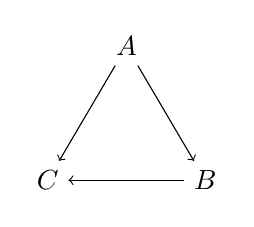
\begin{tikzpicture}
				\node (a) at (1,1.7) {$A$};
				\node (b) at (2,0) {$B$};
				\node (c) at (0,0) {$C$};
				
				\draw[->] (a) -- (b);
				\draw[->] (b) -- (c);
				\draw[->] (a) -- (c);
			\end{tikzpicture}
		\end{center}

		15)$A<C<B \quad A<B$\\
		\begin{center}
			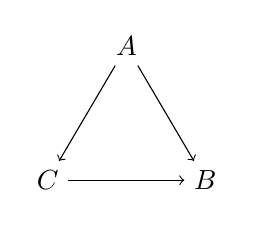
\begin{tikzpicture}
				\node (a) at (1,1.7) {$A$};
				\node (b) at (2,0) {$B$};
				\node (c) at (0,0) {$C$};
				
				\draw[->] (a) -- (c);
				\draw[->] (c) -- (b);
				\draw[->] (a) -- (b);
			\end{tikzpicture}
		\end{center}
		
		16)$B<A<C \quad B<C$\\
		\begin{center}
			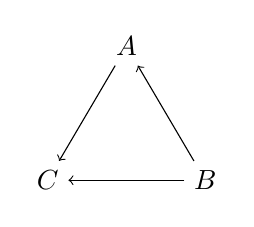
\begin{tikzpicture}
			\node (a) at (1,1.7) {$A$};
			\node (b) at (2,0) {$B$};
			\node (c) at (0,0) {$C$};
			
			\draw[->] (b) -- (a);
			\draw[->] (a) -- (c);
			\draw[->] (b) -- (c);
			\end{tikzpicture}
		\end{center}
		
		17)$B<C<A \quad B<A$\\
		\begin{center}
			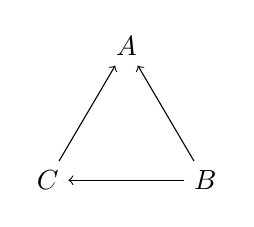
\begin{tikzpicture}
			\node (a) at (1,1.7) {$A$};
			\node (b) at (2,0) {$B$};
			\node (c) at (0,0) {$C$};
			
			\draw[->] (b) -- (c);
			\draw[->] (c) -- (a);
			\draw[->] (b) -- (a);
			\end{tikzpicture}
		\end{center}
		
		18)$C<B<A \quad C<A$\\
		\begin{center}
			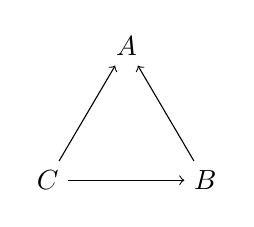
\begin{tikzpicture}
			\node (a) at (1,1.7) {$A$};
			\node (b) at (2,0) {$B$};
			\node (c) at (0,0) {$C$};
			
			\draw[->] (c) -- (b);
			\draw[->] (b) -- (a);
			\draw[->] (c) -- (a);
			\end{tikzpicture}
		\end{center}
		
		19)$C<A<B \quad C<B$\\
		\begin{center}
			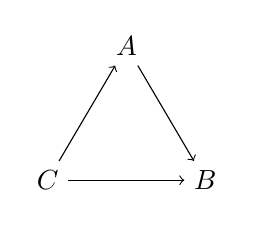
\begin{tikzpicture}
			\node (a) at (1,1.7) {$A$};
			\node (b) at (2,0) {$B$};
			\node (c) at (0,0) {$C$};
			
			\draw[->] (c) -- (a);
			\draw[->] (a) -- (b);
			\draw[->] (c) -- (b);
			\end{tikzpicture}
		\end{center}
		
		\subsection{3}
		1) Не коммутативная операция: \\
		\begin{gather*}
			\begin{pmatrix}
				a_1 & a_2\\
				b_1 & b_2\\
				c_1 & c_2
			\end{pmatrix}
		\cdot
			\begin{pmatrix}
				d_1 & d_2\\
				e_1 & e_2\\
			\end{pmatrix}
		\end{gather*}
		Коммутативность: \\
		Пусть $A = 
		\begin{pmatrix}
		1 & -1\\
		2 & 0\\
		3 & 0
		\end{pmatrix}$ и $B = 
		\begin{pmatrix}
		1 & 1\\
		2 & 0\\
		\end{pmatrix}		
		$\\
		Тогда $A \cdot B =
		\begin{pmatrix}
		-1 & 1\\
		2 & 2\\
		3 & 3
		\end{pmatrix}
		$, но $B \cdot A$ не определен
		Ассоциативность: $(A \cdot B) \cdot C \ne A \cdot (B \cdot C)$\\
		Нейтральный элемент: Единичная матрица\\ \\
		\\
		2) Не ассоциативная операция: \\
		Пусть $a \circleddash b = |a - b|$, тогда:
		Коммутативность: $a \circleddash b = |a - b| = |b - a| = b \circleddash$\\
		Ассоциативность: $(a \circleddash b) \circleddash c \ne a \circleddash (b \circleddash c)$\\
		Рассмотрим $||10 - 7| - 3| = 0 \ne 6 = |10 - |7 - 3||$ \\
		Нейтральный элемент: $a \circleddash 0 = |a|$\\ 
		\\ \\
		3) Без нейтрального элемента: \\
		$x  \star  y = max(x, y)$, для $x, y \in \mathbb{Z}$\\
		Заметим, что наличие нейтрального элемента равносильно наличию минимального числа, что для $\mathbb{Z}$ не верно, при этом \\
		$x \star y = y \star x$ и $(x \star y) \star z = x \star (y \star z)$
		
		\subsection{4}
		1) Заметим, что для класса эквивалетности элемента $a$ верно (далее $M(a)$), что для $\forall b \in M(a): \ M(b) = M(a)$, так как если рассмотреть элемент $c_a \in M(a)$, то $a \sim c_a$, при этом $a \sim b$, откуда $b \sim c_a$. Аналогично для любого элемента $c_b$ из $M(b)$ верно, что $a \sim c_b$.\\
		\\
		Откуда следует, что если $M(a_1) \cap M(a_2) \ne 0$, то для $d \in M(a_1) \cap M(a_2): \quad M(a_1) = M(d),\ M(a_2) = M(d) \Longrightarrow M(a_1) = M(a_2)$\\
		\\
		2) Покажем, что указанное отношение - отношение эквивалентности:\\
		2.1) $x \sim x$: это выполнено, так как элемент находится в том же подмножестве разбиения, что и этот элемент.\\
		2.2) $x \sim y$ $\Longrightarrow$ $y \sim x$: очевидно выполнено\\
		2.3) $x \sim y$ и $y \sim z$ $\Longrightarrow$ $x \sim z$: очевидно выполнено\\
		
		\subsection{5}
		Проверим, что $R$ -- отношение эквивалетности:\\
		1. $f(a) = f(a)$\\
		2. $f(a) = f(b) \Longrightarrow f(b) = f(a)$\\
		3. $f(a) = f(b),\ f(b) = f(c) \Longrightarrow f(a) = f(c)$\\
		\\
		Сопоставим каждому множеству $M$ из $X/R$ значение $f(m)$, где $m$ принадлежит $M$ (нетрудно видеть, что для любых $m$ $f(m)$ будет одинаковым), при этом любой образ будет получен.
		
		\subsection{6}
		Покажем "переносимость" коммутативности, ассоциотивности и наличия нейтрального элемента.\\	
		1)\\
		Если $a * b = b * a$, то $A\overline{ * }B = B\overline{ * }A$, так как $a * b \sim c  \Rightarrow b * a \sim c$  для любых $a$ и $b$ из множеств $A$ и $B$ соотв.\\
		2)\\
		Если $(a * b) * c = a * (b * c)$, то $(A\overline{ * }B)\overline{ * }C = A\overline{ * }(B\overline{ * }C)$, так как $(a * b) * c \sim d  \Rightarrow a * (b * c) \sim d$  для любых $a$, $b$ и $c$ из множеств $A$, $B$ и $C$ соотв.\\
		3)\\
		Если существует такое $e$: $a * e = a$, то есть и $E$: $A\overline{ * }E = A$, так как рассмотрим множество, в котором находится $e$ (пусть это $E_1$), тогда для любого элемента $e_1$ из $E_1$ верно: $a * e_1 \sim a$, так как $a * e \sim a$.\\
		\\
		Примеры: умножение и сложение на $GF_2$
%		
		\subsection{7}
		Заметим, что выполняются симметричность и рефлексивность. ($a + b^{/} = a^{/} + b \to a^{/} + b = a + b^{/};\ a + b = b + a$). Проверим транзитивность:
		\begin{gather*}
		(a_1, \: b_1) \sim (a_2, \: b_2) \Rightarrow a_1 + b_2 = a_2 + b_1 \Rightarrow a_1 - b_1 = a_2 - b_2 \\
		(a_2, \: b_2) \sim (a_3, \: b_3) \Rightarrow a_2 + b_3 = a_3 + b_2 \Rightarrow a_2 - b_2 = a_3 - b_3 \\
		\Rightarrow a_1 - b_1 =  a_3 - b_3 \Rightarrow a_1 + b_3 = a_3 + b_1 \Rightarrow (a_1, \: b_1) \sim (a_3, \: b_3)
		\end{gather*}
		Заметим, что 2 элемента находятся в одном классе эквивалентности если у них одинаковая разность координат, откуда вытекает, что фактор-множество состоит из множеств, каждому из которых можно сопоставить целое число равное разности координат.\\
		Отсюда следует, что покоординатное сложение согласовано с этим отношением эквивалентности, "складывая" элементы из множеств $x$ и $y$ в $x+y$ ($x,y$ -- целые числа, сопоставленные множествам). $(a_1; \: a_1 - x) \ "+" \ (a_2; \: a_2 - y) \: = \: (a_1 + a_2; \: a_1 + a_2 - (x + y))$\\
		Заметим, что мы показали, что покоординатное сложение изоморфно сложению, откуда следует, что для него выполнены все указанные в задаче условия.
		
		\subsection{8}
		Пусть $x = a_1n+ z_1 \equiv z_1$ и $y = a_2n + z_2 \equiv z_2$, причем $z_1 < n$ и $z_2 < n$.\\
		Тогда $x + y = (a_1n+ z_1) + (a_2n + z_2) = (a_1 + a_2)n + z_1 + z_2 \equiv z_1 + z_2 $ \\ \\
		И $x  \cdot  y = (a_1n+ z_1)  \cdot  (a_2n + z_2) = a_{1}a_{2}n^{2} + a_{1}z_{2}n + z_{1}a_{2}n + z_{1}z_{2} =\\
		(a_{1}a_{2}n + a_{1}z_{2} + z_{1}a_{2})n + z_{1}z_{2} \equiv z_{1}z_{2} $
		
		\subsection{9}
		
		\subsection{10}
		Пусть есть 4 вектора: $A(x_{1}, y_{1}, z_{1})$, $B(x_{2}, y_{2}, z_{2})$, $C(x_{1}, y_{1}, z_{3})$, $D(x_{2}, y_{2}, z_{4})$, причем $A \sim C$ и $B \sim D$, где $\sim$ обозначает отношение эквивалентности.\\
		Докажем тогда что $A+B \sim C+D$:
		\begin{gather*}
			(A+B) - (C+D) = 
			\biggl( (x_{1}, y_{1}, z_{1}) + (x_{2}, y_{2}, z_{2}) \biggl) - \biggl( (x_{1}, y_{1}, z_{3}) + (x_{2}, y_{2}, z_{4}) \biggl) = \\
			((x_{1} + x_{2}) - (x_{1} + x_{2}), (y_{1} + y_{2}) - (y_{1} + y_{2}), (z_{1} + z_{3}) - (z_{2} + z_{4})) = \\
			(0, 0, z_{1} + z_{3} - z_{2} - z_{4})
		\end{gather*}
		Т.е. $(A+B) - (C+D) \parallel O_{Z}$, что равносильно $A+B \sim C+D$
		
		
		\subsection{11}
		Пусть есть 4 вектора: $A(x_{1}, y_{1}, z_{1})$, $B(x_{2}, y_{2}, z_{2})$, $C(x_{3}, y_{3}, z_{1})$, $D(x_{4}, y_{4}, z_{2})$, причем $A \sim C$ и $B \sim D$, где $\sim$ обозначает отношение эквивалентности.\\
		Докажем тогда что $A+B \sim C+D$:
		\begin{gather*}
			(A+B) - (C+D) = 
			\biggl( (x_{1}, y_{1}, z_{1}) + (x_{2}, y_{2}, z_{2}) \biggl) - \biggl( (x_{3}, y_{3}, z_{1}) + (x_{4}, y_{4}, z_{2}) \biggl) = \\
			((x_{1} + x_{2}) - (x_{3} + x_{4}), (y_{1} + y_{2}) - (y_{3} + y_{4}), (z_{1} + z_{2}) - (z_{1} + z_{2})) = \\
			(x_{1} + x_{2} - x_{3} - x_{4}, y_{1} + y_{2} - y_{3} - y_{4}, 0)
		\end{gather*}
		Т.е. $(A+B) - (C+D) \perp O_{Z}$, что равносильно $A+B \sim C+D$
		
		\subsection{12}
		A)\\
		(заметим, что $f$: $x \to x+1$ для множества целых чисел; является биекцией, но $R$ не является отношением эквивалентности)\\
		\\
		Докажем, что если $f$ -- объединение биекций конечных непересекающихся подмножеств множества $X$, объединение которых равно $X$, то $R$ -- отношение эквивалентности. Назовём псевдоклассом эквивалентности с элементом $x$ следующее множество элементов: $x, f(x), f^2(x), ... \ $. Заметим, что так как $x$ принадлежит конечному подмножеству, относительно которого $R$ -- биекция, то существует такое $k: f^k(x) = x$, откуда псевдокласс эквивалентности конечен, при этом нетрудно видеть, что если $y$ принадлежит псевдоклассу относительно $x$, то и наоборот, поэтому разбиение множества $X$ на псевдоклассы эквивалентности однозначно определено. Нетрудно видеть, что для любых 2х элементов из одного класса псевдоэквивалентости равны относительно $R$, при этом это не верно для 2х элементов из разных классов, откуда следует, что $R$ -- отношение эквивалентности, классы которого равны псевдоклассам.
		\\ \\
		B)\\
		Назовём циклом в $f$ такое упорядоченное с точностью до сдвига множество попарно различных элементов $[a_1, a_2, ... , a_n]$, что $\forall i$ принадлежащего вычетам по модулю $n: a_{i+1} = f(a_i)$. Заметим, что отсутствие циклов в $f$ (1) эквивалентно тому, что $R$ -- отношение частичного порядка (2): \\
		Заметим, что $R$ рефлексивно и транзитивно, поэтому $R$ -- отношение частичного порядка (2) $\Leftrightarrow$ $R$ -- антисимметрично (3) \\
		не (1) $\Rightarrow$ не (3) \\
		Рассмотрим цикл $[a_1, a_2, ... , a_n]$, тогда $a_1 R a_2$ -- истина, и $a_2 R a_1$ -- истина, откуда $R$ -- не антисимметрично, так как $a_1 \ne a_2$ \\
		не (3) $\Rightarrow$ не (1) \\
		Рассмотрим пару $a_1, a_2: \quad a_1 R a_2 \cap a_1 R a_2 \ \Leftrightarrow \ a_1 = a_1$. То есть существуют такие $k_1, k_2: \quad a_2 = f^{k_1}(a_1), a_1 = f^{k_2}(a_2)$, откуда следует, что существует следующий цикл: $[a_1, f(a_1), ... , f^{k_1 - 1}(a_1), a_2, f(a_2), ... , f^{k_2 - 1}(a_2)]$
		\\
		Теперь заметим, что если есть цикл, то указанное в условии пересечение ненулевое, а именно является объединением "чего-то" и этого цикла. Нетрудно видеть, что цикл переходит сам себя. Отсюда следует, что если пересечение пусто, то цикла нет $\Rightarrow$ $R$ -- отношение частичного порядка
		\\
		Пусть $X$ -- множество из одного элемента, тогда пересечение равно этому элементу, но при этом $R$ -- отношение частичного порядка.\\
		\\
		В обратную сторону: \\
		Докажем, что если $R$ -- отношение частичного порядка, то пересечение $f^k(M) = 0$ для любого конечного подмножества $M$ без неподвижных элементов. Эквивалентное утверждение: если нет циклов, то пересечение $f^k(M) = 0$. Пусть есть подмножество с ненулевым пересечением, тогда рассмотрим это пересечение. Оно переходит в себя $\Rightarrow$ есть цикл, так как множество конечное. Поэтому если нет циклов, то пересечение пусто.
		
		\subsection{13}
		Заметим, что выполнена рефлексивность, выбрав тождественные биекции.\\
		Выполнена транзитивность, так как есть такие $\phi_1, \phi_2, \psi_1, \psi_2: \quad \psi_1 \circ f = g \circ \phi_1,\ \psi_2 \circ h = f \circ \phi_2 \quad \Rightarrow \\
		\psi_1 \circ \psi_2 \circ h = \psi_1 \circ f \circ \phi_2 = g \circ \phi_1 \circ \phi_2$, откуда есть такие биекции для $g$ и $h$.\\
		Выполнена симметричность, так как $\psi \circ f = g \circ \phi \ \Rightarrow \ \psi^{-1} \circ \psi \circ f \circ \phi^{-1}  = \psi^{-1} \circ g \circ \phi \circ \phi^{-1}  \ \Rightarrow \
		f \circ \phi^{-1} = \psi^{-1} \circ g$\\
		Поэтому $R$ -- отношение эквивалентности. 
		\\
		Заметим, что если $f$ и $g$ такие, что их образы состоят из одного элемента (пусть для $f$ это $e_f$, для $g$ -- $e_g$, то заметим, что биекция $k$: $Y \to Y$, переводящая $e_f \to e_g,\ e_g \to e_f$, остальные элементы неподвижны, является такой, что $k \circ f = g$, поэтому $fRg$.\\
		\\
		Заметим, что каждому классу эквивалентности относительно $R$ можно сопоставить диаграмму Юнга фиксированного веса. Так, если рассмотреть количество прообразов у каждого образа, отсортировать их по убыванию, и поставить в каждую строку некое количество квадратов, равное количеству прообразов. Соответственно модуль образа равен количеству строк в сопоставленной диаграмме Юнга. Диаграмм Юнга, состоящих из двух строк суммарной массы $n$, ровно $[ \frac{n}{2} ]$. Так как есть $[ \frac{n}{2} ]$ спообов выбрать выбрать из $n$ не меньшее($\geqslant$) слагаемое.
		
		\subsection{14}
		Заметим, что каждому множеству из фактормножества $\mathbb{R}/\mathbb{Z}$ можно сопоставить точку из отрезка $[0,1)$ Покажем, что есть биекция между $[0,1)$ и $[0,4)$ (домножение на 4) и между $[0,1)$ и $[0.1]$ (сопоставим точкам вида $\frac{1}{2^k}$ точку $\frac{1}{2^{k-1}}$). $[0,1) + [1,2) + [2,3) + [3,4) = [0,4)$. Пусть $x$ принадлежит $[0,1)$, сопоставим ей точку $(1 - x; \sqrt{2x - x^2})$, таким образом $[0,1) \ \to$ часть окружности из первой четверти ($M_1$). Аналогично для остальных полуинтервалов.
		
		\subsection{15}
		Заметим, что композиция - точки вида ($2 cos \phi; 3 sin \phi$) для всех углов $\phi$. При этом $cos^2 \phi + sin^2 \phi = 1$, откуда если $2 cos \phi = x, 3 sin \phi = y$, то $\frac{x^2}{4} + \frac{y^2}{9} = 1$, что есть эллипс.
		
		\subsection{16}
		1)\\
		Заметим, что\\
		1.1) Из $A$ в $A$ можно попасть минуя мосты\\
		1.2) Если можно пройти из $A$ в $B$, минуя мосты, то по этому же пути можно пройти и в обратную сторону из $B$ в $A$\\
		1.3) Если можно пройти из $A$ в $B$ и из $B$ в $C$, минуя мосты, то из $A$ в $C$ можно попасть через $B$ и тогда мы не пройдем ни по одному мосту\\
		$\Longrightarrow$ эта операция является отношением эквивалентности\\
		\\ \\
		2)\\
		Пусть в графе $k$ мостов, докажем тогда что в нем $k+1$ класс эквивалентности:\\
		2.1) Пусть классов эквивалентности $< k+1$, тогда после убирания всех мостов, какой-то класс эквивалентности соответствует нескольким компонентам связности, а по (3) класс эквивалентности не может соответствовать $\geqslant 2$ компонентам связности\\
		2.2) Пусть классов эквивалентности $> k+1$, тогда какие-то 2 класса эквивалентности соответствуют одной компоненте связности, но при этом для них выполнен (1) $\Longrightarrow$ противоречие
		\\ \\
		3)\\
		Уберем все мосты, тогда заметим, что образовался $k+1$ связанный граф, так как при убирании каждого моста добавлялся ровно 1 элемент свзности(если элемент не добавлялся, то убранное ребро - не мост, а $\geqslant 2$ элементов добавиться не могло, так как каждое ребро связывает ровно 2 вершины). Заметим, что если класс эквивалентности не связный граф, то мы можем рассмотреть 2 его элемента, принадлежащие разным компонентам связности, но очевидно, что тогда из одной нельзя пройти в другую(так как они в разных компанентах связности), но тогда, если рассматривать изначальный граф, путь, соединяющий эти две вершины, обязан проходить через мост - простиворечие, так как если все пути из одной вершины в другую проходят через мост, то они принадлежат различным классам эквивалентности.
		\\
		\subsection{17}
		Рассмотрим рокады, для них по условию выполнено:\\
		1) Каждая рокада эквивалентна самой себе\\
		2) Две различные рокады эквивалентны, если при их удалении
		граф становится несвязным\\
		Тогда чтобы показать что это отношение эквивалентности, нужно показать что если $a \sim b$ и $b \sim c$, то $a \sim c$. \\
		3)Действительно, заметим что каждая рокада относится к какому-то одному классу эквивалентности(так как если она относится к нескольким классам эквивалентности, то мы можем рассмотреть любые 2 из них, назовем их $a_1$ и $a_2$ -- удалим выбранную рокаду и рокаду из $a_1$, тогда мы можем заметить, что $a_2$ остался связным(хотя в нем и появился мост), но тогда мы можем заметить, что $a_1$ тоже остался связным, так как ккждая изего половин осталось соединенной с $a_2$, а $\Longrightarrow$ при удалении 2 рокад из $a_1$, граф не потерял связность $\Longrightarrow$ два удаленных ребра не были рокадами), тогда заметим что $a$ с $b$ и $c$ с $b$ в одном классе эквивалентности, а следовательно и $a$ с $c$ в одном классе эквивалентности и $a \sim c$. \\
		Тогда заданное отношение эквивалентности на рокадах действительно является отношением эквивалентности. %что просили то и доказал, формулируйте условие получше
		\\ \\
		Заметим что если построить n-угольник, вершины которого - вершины графа, а стороны - ребра, то у полученного графа будет только один класс эквивалентности(что можно проверить по первому пункту задачи). Также заметим, что если соединить 2 многоугольника по вершине, то мы получим 2 класса эквивалентности. Тогда будем соединять многоугольники(с любым числом вершин, необязательно одинаковым) по вершинам(т.е. у 2 многоугольников будет общая вершина), соединять будем в цепочку, хотя остальные конструкции тоже работают. Рассмотрим цепочку из $n$ многоугольников - у неё будет $n$ классов эквивалентности(по одному на каждый многоугольник)
		\\
		Пусть в одном из классов эквивалентности $k$ рокад, удалим их все - русть мы удаляли их в каком-то порядке, тогда после удаления одной рокады все остальные рокады стали мостами $\Longrightarrow$ приудалении каждого из них количсетво компанент связности увеличивалось на 1, тогда после удаления всех мостов мы получили $k-1$ новую компаненту связности + был еще изначальный граф, ребра которого мы удаляли - следовательно после удаления $k$ рокад мы получили $1 + (k-1) = k$ компанент связности, что и требовалось.